\documentclass[utf8, 11pt]{beamer}
\usepackage{verbatim}
\usepackage{color}
\usepackage{graphicx}
\usepackage{alltt}
%\usepackage{hyperref}
%\hypersetup{colorlinks=true, urlcolor=cyan}
\hypersetup{urlcolor=cyan}

\mode<presentation>
{
  \usetheme{default}
}

\usepackage[english, russian]{babel}
\usepackage{graphicx}
\usepackage{colortbl}
\usepackage{listings}

\newcommand{\rsb}{\cellcolor[gray]{0.85}}
\newcommand{\nam}[1]{\texttt{#1}}

\setbeamertemplate{navigation symbols}{} 

\author[ ]{Карташов Д. А., Орлов А. В., Азаров А. И. \\ Руководитель: Кринкин К. В.}

\title[Virtual HSM]{Разработка виртуального HSM для платформы Linux}

\institute[СПбАУ]
{
  Кафедра математических и информационных технологий\\
  Санкт-Петербургский Академический университет
}

\date{ }

\subject{Talks}

\useoutertheme{infolines}
\setbeamertemplate{headline}{}

\begin{document}

\begin{frame}
  \titlepage
\end{frame}

\begin{frame}{Введение}

Криптография в приложениях:
\begin{itemize}
\item хранение секретных данных
\item вычисления с их использованием
\end{itemize}

\vspace*{\fill}

Проблемы безопасности:
\begin{itemize}
\item компрометация секретных данных
\end{itemize}

\vspace*{\fill}

Решение:
\begin{itemize}
\item исключить попадание секретных данных на диск и/или в память компьютера
\end{itemize}

\vspace*{\fill}

\end{frame}

\begin{frame}{Цели и задачи проекта}

\begin{block}{Цель}
Разработать решение, предоставляющее функциональность HSM в виртуальном окружении
\end{block}

\vspace*{\fill}

\begin{block}{Задачи}
\begin{itemize}
\item \textcolor{gray}{поиск и анализ существующих решений;}
\item \textcolor{gray}{изучение стандартов HSM;}
\item разработка прототипа VHSM:
\begin{itemize}
	\item клиентский API;
	\item защищенное хранилище;
	\item транспорт;
\end{itemize}
\item формирование конечного продукта:
\begin{itemize}
	\item система сборки;
	\item unit и интеграционные тесты;
	\item пакетирование.
\end{itemize}
\end{itemize}
\end{block}
\end{frame}

\begin{frame}{Общая архитектура решения}
\begin{center}
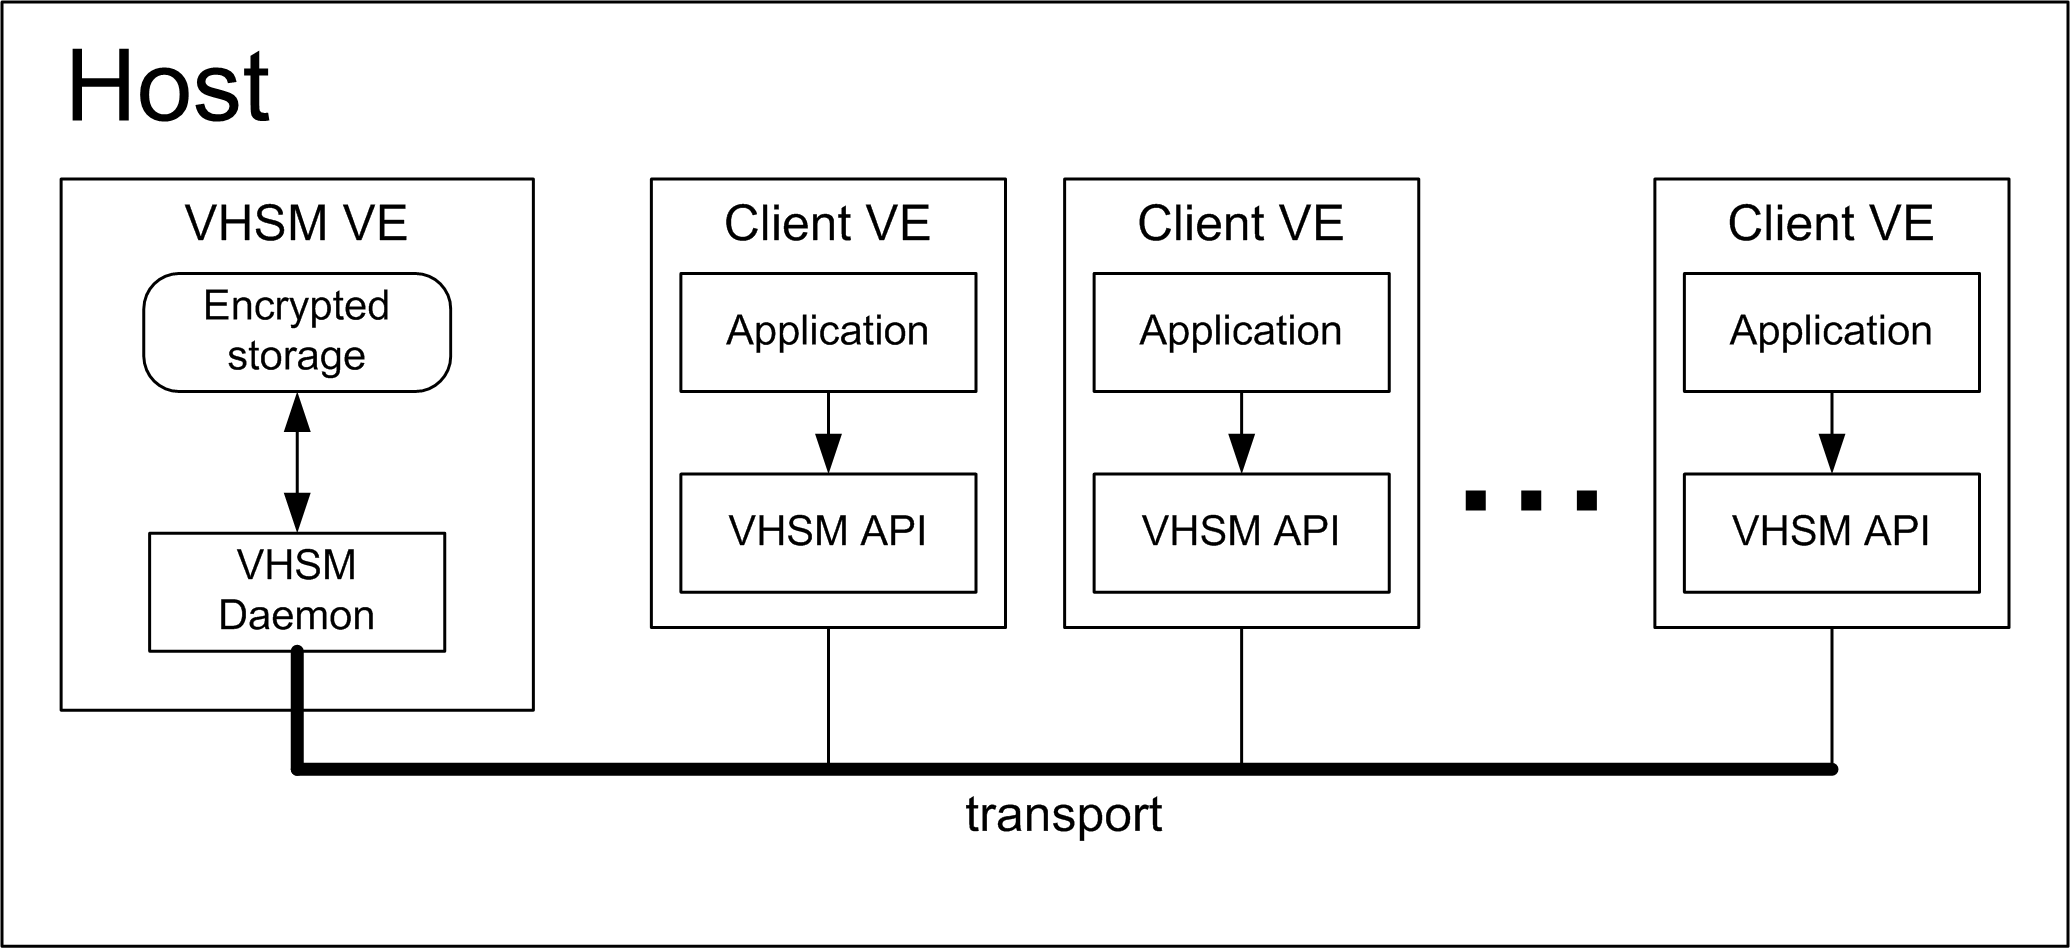
\includegraphics[width=0.95\paperwidth]{img2}
\end{center}
\end{frame}

\begin{frame}{Основные компоненты}
\begin{itemize}
\item {\bf Transport}
	\begin{itemize}
		\item пересылка сообщений
		\item идентификация контейнеров
	\end{itemize}
\item {\bf VHSM API}
	\begin{itemize}
		\item передача запросов на выполнение криптографических операций через транспорт
		\item получение результатов операций
	\end{itemize}
\item {\bf VHSM daemon}
	\begin{itemize}
		\item аутентификация
		\item выполнение криптографических операций с использованием секретных данных
	\end{itemize}
\item {\bf Encrypted storage}
	\begin{itemize}
		\item хранение секретных данных пользователя
	\end{itemize}
\end{itemize}

\end{frame}

\begin{frame}[fragile]
\frametitle{Transport}
\begin{itemize}
\item протокол --- \texttt{Google Protobuf}
\item реализован на основе netlink
\end{itemize}
\begin{center}
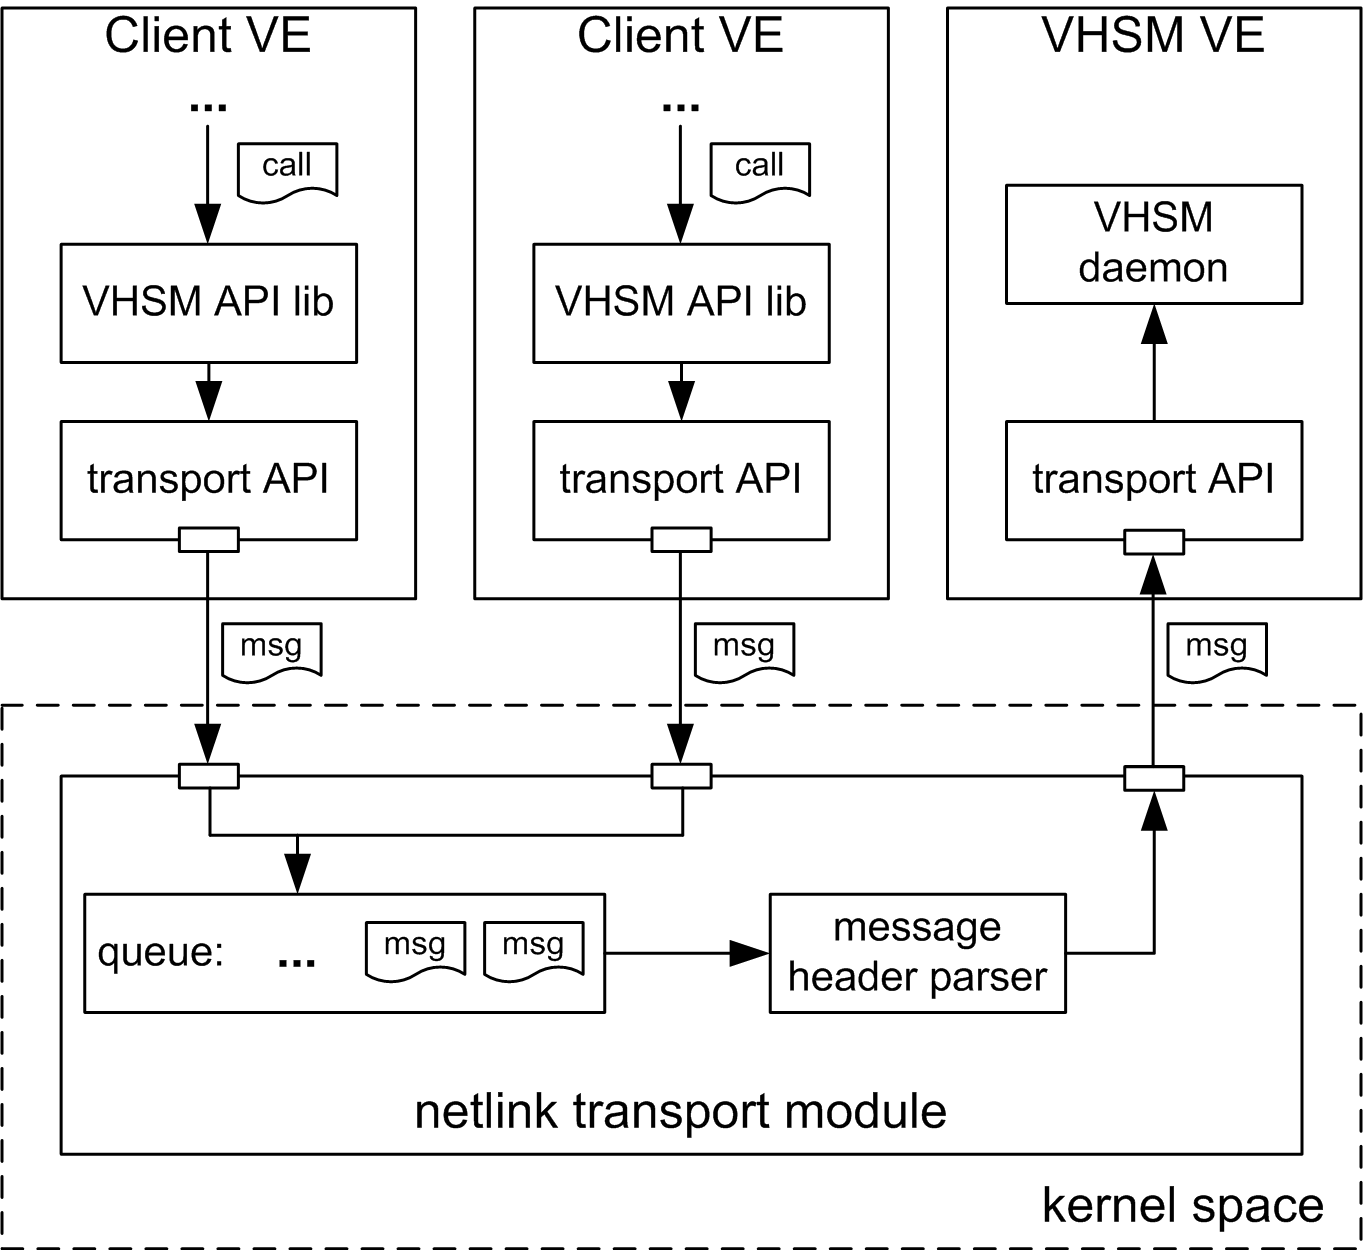
\includegraphics[scale=0.65]{img4}
\end{center}
\end{frame}

\begin{frame}{VHSM API}

\begin{itemize}
\item управление сессиями
\begin{itemize}
\item открытие/завершение сессии;
\item аутентификация пользователя;
\end{itemize}

\item управление ключами
\begin{itemize}
\item импорт;
\item генерация;
\item удаление;
\end{itemize}

\item хэширование и МАС
\begin{itemize}
\item стандартные функции: \texttt{init, update, final}
\end{itemize}
\end{itemize}

\vspace*{\fill}

\end{frame}

\begin{frame}{VHSM daemon \& encrypted storage}

\begin{itemize}
\item вычисление криптографических функций
\item хранение пользовательских данных:
	\begin{itemize}
	\item база данных SQLite;
	\item пользовательские ключи хранятся в зашифрованном виде;
	\item шифрование AES в режиме GCM;
	\item ключ шифрования генерируется функцией PBKDF2 на основе пароля пользователя;
	\end{itemize}
\end{itemize}
\vspace*{\fill}
\end{frame}

\begin{frame}{Пример использования}
\begin{center}
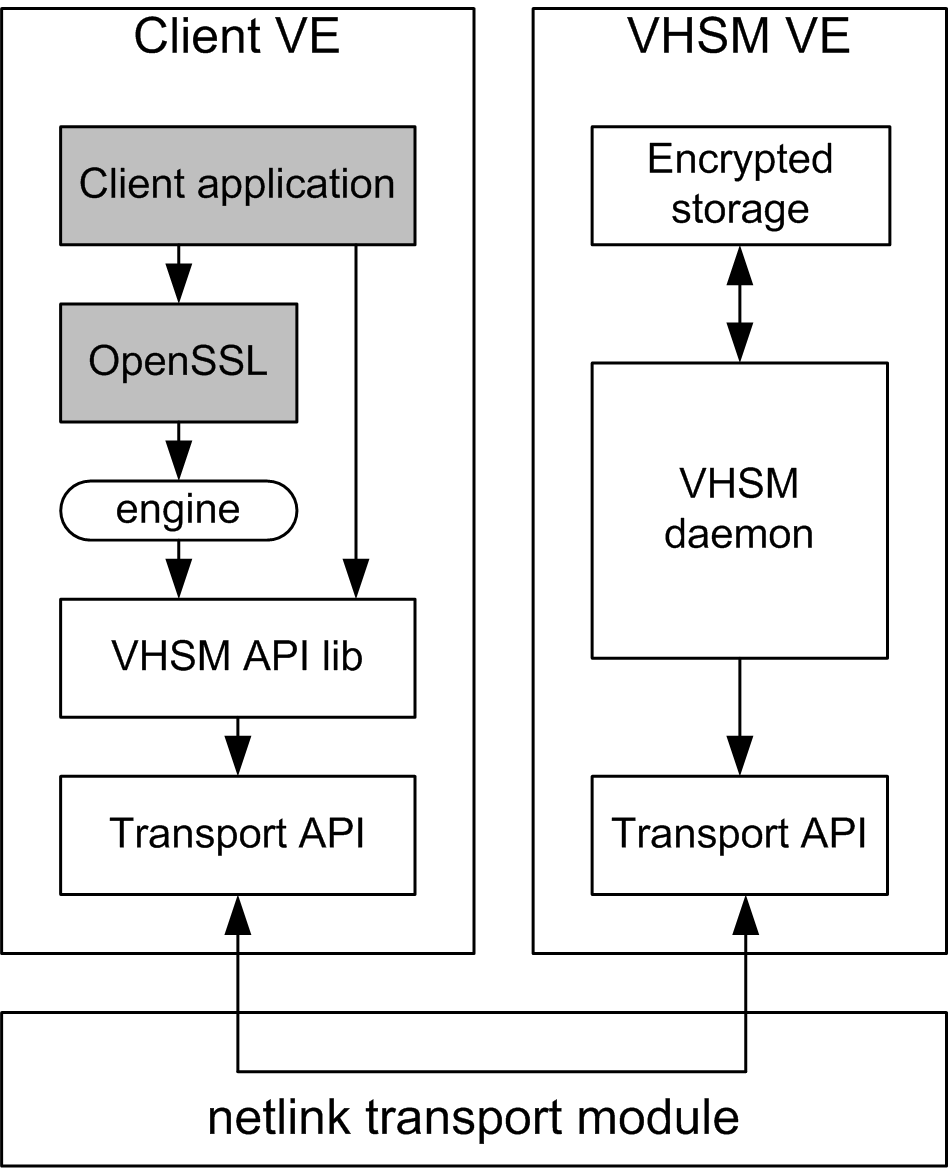
\includegraphics[scale=0.75]{img3-2}
\end{center}
\end{frame}

\begin{frame}{Тестирование}
\begin{itemize}
\item Unit-тесты
\item Интеграционные тесты:
	\begin{itemize}
	\item установка и инициализация контейнеров;
	\item создание пользователя;
	\item вход и выход из системы;
	\item операции с ключами;
	\item HMAC.
	\end{itemize}
\end{itemize}
\vspace*{\fill}
\end{frame}

\begin{frame}{Система сборки и пакетирование}
\begin{itemize}
\item Система сборки:
	\begin{itemize}
	\item cmake;
	\end{itemize}
\item Генерация пакетов:
	\begin{itemize}
	\item rpm;
	\item deb;
	\end{itemize}
\item Пакеты:
	\begin{itemize}
	\item client;
	\item server;
	\item host.
	\end{itemize}
\end{itemize}
\vspace*{\fill}
\end{frame}

\begin{frame}{Итоги и планы}

Итоги:
\begin{itemize}
\item реализована система, состоящая из нескольких компонентов:
\begin{itemize}
	\item клиентская библиотека;
	\item транспортный модуль;
	\item VHSM и хранилище;
\end{itemize}
\item внедрена система сборки;
\item проведены unit и интеграционные тесты;
\end{itemize}

\vspace*{\fill}

Планы на будущее:
\begin{itemize}
\item расширение функциональности VHSM;
\item введение прав пользователей и уровней доступа.
\end{itemize}

\vspace*{\fill}

\end{frame}

\begin{frame}{Ссылки}
\begin{itemize}
\item Репозиторий проекта:

\url{https://github.com/OSLL/vhsm}

\item wiki проекта:

\url{http://dev.osll.ru/projects/vhsm/wiki}
\end{itemize}

\vspace*{\fill}

\end{frame}

\end{document}
